\documentclass[english]{beamer}
\usepackage[utf8,latin9]{inputenc}
%%\usepackage[latin9]{inputenc}
\usepackage[T1]{fontenc}
\usepackage{babel}

\usepackage{beamerthemesplit}
\usetheme{Warsaw}
\beamertemplatetransparentcovered

\title{pg\_staging}
\author{Dimitri Fontaine}
\date{May, 20 2010}

\begin{document}

\frame{\titlepage}

\section*{Outline}
\frame{
  \frametitle{Table of contents}
  \tableofcontents
}

\section{Bird Eye View}

\frame{
  \frametitle{pg\_staging in one image}

  This image seems not to help people at all, from my blog's readers, so I
  figured I had to show it up somehow.

  \begin{center} 
    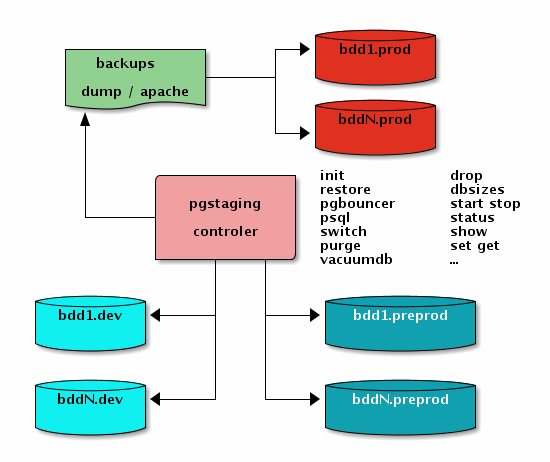
\includegraphics[height=1.6in]{pg_staging.png}
  \end{center}   
}

\section{Current dependencies}

\frame{
  \frametitle{What do you need for pg\_staging to run}

  So for \texttt{pg\_staging} to work you need to install:

  \begin{itemize}
  \item<1-> \texttt{apache} for publishing your backups,
    \texttt{database\_YYYY-MM-DD}
  \item<2-> \texttt{pgbouncer} to switch database without messing with the
    applications setup
  \item<3-> some non interactive \texttt{ssh} facility
  \item<4-> a \texttt{sudo} account, typically user \texttt{pgstaging}
  \item<5-> the \textit{pg\_staging client} on each machine where you restore
  \end{itemize}
}

\section{Quick Setup}

\frame{
  \frametitle{Setting up can get engaging}

  So for \texttt{pg\_staging} to work you need to install:

  \begin{itemize}
  \item<1-> Setup \texttt{apache} to serve the backup files
  \item<2-> Setup \texttt{pgbouncer} to expose the \texttt{postgres} database
  \item<3-> Setup \texttt{ssh} and \texttt{sudo} and install the \textit{client}
  \item<4-> Use the console!
  \end{itemize}
}

\section{Services}

\frame{
  \frametitle{Now what}

  \begin{itemize}
  \item init, dump, redump, restore, drop, switch
  \item purge, vacuumdb, load, createdb, fetch, presql, postsql
  \item databases backups dbsize dbsizes psql show search\_path
  \item pgbouncer pause resume
  \item londiste stop start status restart
  \item get set
  \item nodata catalog triggers
  \end{itemize}
}

\frame{
  \frametitle{What's the watch saying?}

  If we have some time left and I still can breeze, let's talk some more about:

  \begin{itemize}
  \item catalog and triggers command
  \item TODO: fetching backups method, bypassing apache for local files
  \item \texttt{pg\_staging 0.12} should be simplifying the setup needs
  \end{itemize}

}

\frame{
  \frametitle{Conclusion}

  \begin{center} 
    NEXT!
  \end{center}  
}

\end{document}
